This chapter describes the evolution of frame format proposed in \ref{ch:proposal}. Also, it describes the reason for each change based on better understanding the needs of the other teams and the problems in the development. Figure \ref{Interface} is a diagram of our interaction with the other teams that make up this network. 
\begin{figure}[ht]
    \centering
    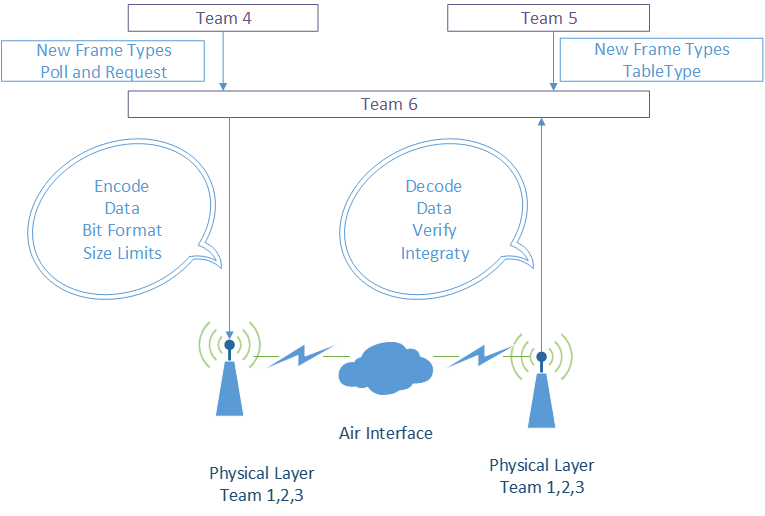
\includegraphics[width=0.8\textwidth]{Interface_diagram.PNG}
    \caption{Diagram of how Module 6 interfaces with the rest of the network}
    \label{fig:Interface}
\end{figure}


\section{MAC Frame Construction}
The structure of a frame is affected by many factors. In this project, in order to make the design as simple as possible, we put the simplicity as the primary factor. That is when there is a conflict between the simplicity and efficiency or other factors, we choose the simplicity, the efficiency or there factors is less important. This section will introduce all the sections of the frame structure one by one in details. 

\subsection{The Services Provided by MAC Layer}

The basic service of our MAC layer is to move a frame from end to end. Basically saying, the MAC layer is implemented below the application layer and above the physical layer. The application layer generates the data and passes it below to the MAC layer. The MAC layer encapsulates the data with a header and a checksum tailer, then pass it to the USRP N210, which is the physical layer. Possible services that can be offered by our MAC layer include: 

\subsubsection{Framing} The MAC layer encapsulates data received from up layers within a MAC frame before transmission to the physical layer. A frame consists of a data field, in which the the data is inserted, and a number of header fields. 
\subsubsection{Reliable delivery} For end-to-end links that have a single sender at one end of the link and a single receiver at the other end of the link, the MAC protocol is simple. When a MAC protocol provides reliable delivery service, it guarantees to move each data across the link without error.  The reliable delivery service can be achieved with acknowledgments and retransmissions. In other words, the MAC layer focuses an end-to-end retransmission if the data is corrupted. 
\subsubsection{Error detection} The receiver can incorrectly decide that a bit in a frame is zero when it was transmitted as a one, and vice versa. Such bit errors are introduced by signal attenuation and electromagnetic noise. The MAC layer protocol provide a mechanism to detect such bit errors, which is done by having the transmitter include error-detection bits in the frame, and having the receiver perform an error check. In this project, we adopted CRC-8 to perform the error detection. 
\subsubsection{Routing Protocols} As the cellular network in the project has no network layer, the MAC layer has to deal with the end-to-end routing protocols. During the process, many protocols have been considered. More details are provided below. 




\subsection{Error-Detection Techniques}
During the communication, it is important to detect the corruption of bits in a MAC frame sent from one node to another node. At the sender, to be protected against bit errors is augmented with error-detection bits, CRC-8 in the project. Typically, the frame to be protected includes not only the data passed down from the application for transmission, but also MAC layer header information. Both data and CRC-8 are sent to the receiver in a MAC frame. At the receiver, a sequence of bits, data and CRC-8 is received. If the CRC-8 differ from the original CRC-8 at the sender, this means there are bit flips in transit.  In this project, we adopted CRC-8 (Cyclic Redundancy Checks-8bits). 

\subsubsection{Cyclic Redundancy Check (CRC-8)}

CRC-8, also known as polynomial codes, is used widely in today's communication networks. For CRC-8, it is possible to view the bit string to be sent as a polynomial whose coefficients are the 0 and 1 values in the bit string, with operations on the bit string interpreted as polynomial arithmetic. The algorithm of CRC-8 is beyond the limit of this report, we use CRC check library of MATLAB directly. 

Before sending the frames, the sender performed CRC check to the header and data respectively and attached the result in the frame. When the receiver received the frame, it performed CRC check again and compare the results with the original CRC results. If the results are the same, which means both the header and the receiver are intact. Otherwise, if the results are different, this means the frame has been corrupted during the transmission. The receiver will drop the corrupted frames. When the timer of the transmitter timeout, the transmitter will send the same frame again to the receiver. 

In order to implement the CRC function, we add 1 byte CRC-8 checksum at the end of the header and another CRC-8 checksum at the end of the data. According to the requirement of the CRC check library in MATLAB, we have to append the CRC checksum at the end of each corresponding section. 



\subsection{Proposals of MAC Frame Types based on Different Routing Protocols}

Basically, the frame should contains at least the sender ID and the receiver ID in order to implement the routing protocols. However, as for the wireless communication, the routing protocol becomes more difficult than wired communication networks. There are several wireless routing protocols in today's network, we will discuss each of them one by one. 

\subsubsection{Ad-hoc based routing protocols}
First, we consider to borrow the idea of the ad-hoc routing protocols. For ad-hoc mode, the frame contains four addresses in the header. So in our MAC frame, there are four addresses too. In addition to the Sender UE ID, Receiver UE ID, we add Sender BS ID, and Receiver BS ID. The sender will send the frame based on the information of Sender ID and Receiver ID, and the base station forwards the frames based on the information of Sender/Receiver BS ID. The disadvantages of this protocol is obvious. First, the frame is very long due to the existence of four IDs, which go against the simplicity requirement. Second, using four addresses may induce redundant information to the transmission. Take a user sender UE for example, when the UE wants to transmit frames, all it needs is the Sender UE ID and the destination UE ID, the information of Sender BS ID and Receiver ID is unnecessary. Based on the above consideration, we did not adopt the this pan.


\subsubsection{Infrastructure based Wi-Fi routing protocols}

The second mechanism we have considered is the routing idea of infrastructure Wi-Fi. The infrastructure Wi-Fi uses three addresses in the frame header. So in our MAC frame header, there are three addresses. In addition to the Sender UE ID and the Receiver UE ID, we add Next Stage section to the head. Take a communication from UE1 to UE3 for example, UE1 create the frame and put UE1 into the sender ID and UE3 in the receiver ID. As the next hop is BS1, so UE1 put BS1 into the Next Stage section. When BS1 received the frame from UE1, BS1 check the Next Stage content, if the Next Stage is not BS1, BS1 will discard the frame. Otherwise, if the Next Stage is BS1, BS1 will check the receiver ID and the address table. From the address table, BS1 know the next hop is BS2, the destination is UE3, so BS1 changes the content of the Next Stage from BS1 to BS2 and transferred the frame to BS2. Similarly, BS2 removes its ID from the Next Stage section when received the frame and updates it to UE3 then transmit it to UE3. 

This protocol could achieve the routing protocol and the structure of the frame is not so complicated. However, the nodes must change the value of the Next Stage field every hop, also this requires a complicate address table at each node. Based on the simplicity principle, we did not accept this protocol.



\subsubsection{Ethernet based routing protocols}

Even though Ethernet is wired network, we can still borrow the idea of its switching protocol. In an Ethernet, the switch has a switching table. The table uses the MAC address as the ID and different switch interface determine the routing path. For the project, we adopted this idea, which does not require extra sections in the header. In other words, only Sender ID and Receiver ID is enough. The Base stations in the network act like the switch in the Ethernet. We created the address table only for BS1 and BS2, because only base stations will care about the routing protocols. The UEs just need to send the frames to the BS and leave the rest of routing affair to Base stations. When the base station receives a frame, it will check the destination ID and find the corresponding channel or transmission protocol corresponding to the destination ID. Then the BS will know how to transmit the frame to next hop. 

The advantages of this routing protocols are obvious. First, we do not need to add more address types to the header. In addition, the UEs do not need to worry about the routing direction. All the UEs need to do is send frames no matter what the destination is to the Base station,which is physically closed to the UEs.  Therefore, we adopted this protocol. 




\subsection{Frame Size}
In order to guarantee the quality of the transmission, it is often to add some non-sense bits, usually zeros, to the frame. We call this type of non-sense bits as paddings. In addition, the unreliable wireless channel may also induce paddings. Based on those consideration, we set a maximum size for all MAC frames of 240 bytes, i.e., 1920 bits. When the receiver receives an frame, it will know how long the frame is and then allows us to cut off the padding added by the physical layers.  The Frame Size section in the header is 1 byte. 


\subsection{Frame Type}

Another factor we need to consider is the type of the frames. As we cannot transmit data over the whole networks only rely on the data frames, we need more types of frames. For those frames that are not data frames, we call them control frames. Control frames are used to implement different control functions. One of the most popular control frames is the ACK frame. ACK frame is used to inform the sender that the frame is delivered successfully. Any factors result in a frame corrupt or loss will prevent the receiver sending ACK frames. In other words, only when the sender receive an ACK from the receiver, can it send the next frame. 

In this project, there are four more types of control frames including Polling request/respond control frames, address control frame, INVALID frame. Polling request/respond frames are used by Module 4 to implement Polling functions. The address control frame is used by Module 5 to perform address tables update ability. All the other frames that cannot be recognized are belong to the INVALID frames. Whenever an INVALID frame is received, the nodes will do nothing but discarding the frame. 

\begin{table}
\begin{center}
\begin{tabular}{| c | c | c |}
  \hline                       
  Data type & Binary & decimal \\
  \hline
  DATA & 1111 0000 & 240 \\
  ACK & 1111 1111 & 255\\
  INVALID & 0000 0000 & 0\\
  \hline  
\end{tabular}
\end{center}
 \caption{The ID of Different Frame Types}
	\label{tab:frametype}
\end{table}

One thing needs to mention is that the ID of the frame type is not given by random. We apply the Hamming distance theory into this, as shown in  \ref{tab:frametype}. The Hamming distance between two rings of equal length is the number of positions at which the corresponding symbols are different. It measures the minimum number of substitutions required to change one string into the other, both e minimum number of errors that could have transformed one string into the other. 

For example, if we set the type of the data frame as 1, which in binary is 0000 0001. Then we set the type of the INVALID frame as 0, which in binary is 0000 0000. During the transmission, because of the noise or other factors, the bits may be flipped. If the last bit of the data frame is flipped, the receiver will consider this frame is INVALID, and the probability is up to 0.125, which is a high chance. Therefore, if we set the type of the data frame is 240, which in binary is 1111 0000. The hamming distance between the data frame and the INVALID frame is 4, this ensures a much lower probability for the data frame to flip into INVALID types. The later sections will show that since we keep a large hamming distance between each frame types, the correctness gains a great improvement. 


\subsection{Final Decision of Frame Structure}



The proposed frame format in \ref{ch:proposal} had all the necessary fields and some removed to keep the model simple
The final frame format is  shown in \ref{tab:finalFrame}.

\begin{table}
\begin{center}
\begin{tabular}{| c | c | c | c | c | c | c | }
  \hline                       
  Frame Type & Receiver UE & Sender UE & Data Size & Header CRC & Data & Data CRC\\
  \hline
	1 Byte & 1 Byte & 1 Byte & 1 Byte & 1 Byte & 1 to 234 Bytes & 1 Byte\\
  
  \hline  
\end{tabular}
\end{center}
 \caption{Final Frame Format}
	\label{tab:finalFrame}
\end{table}

\section{Transmission and reception process}
%Rebecca

Developing a frame format for transmission through the cellular network is only one part of the end-to-end requirements of data transmission. There must be a system put in place that transfers the data frame between devices and ensures that it gets to the proper receiver. Once at the receiver there should be a check to ensure that the data was received correctly. The reception of a correctly transmitted data frame should return a control frame, ACK, to the sender.  This allows the sending UE to be certain that the data was received correctly and allows it to resend the data frame if the ACK is not received. Just like the data frame, the ACK will have to be properly routed through the network. 

\subsection {Routing}

The network is initialized by Teams 4 and 5 who create a table of the UEs to which each BS has connected. Each UE will always transmit to the same BS, so the data frame can be automatically be sent to the initial BS in the appropriate timeslot.  To determine the routing path at the BS we need to compare the receiver ID field with the IDs in the table and identify if the receiver is connected to the initial cell or if the data frame will need to be sent between cells. If it is sent to the second BS, the data frame will undergo the same routing check again before being sent to the device specified by the receiver. The response ACK will follow the reverse path with all of the same checks at the BS(s). The path through the BSs and UEs is depicted in Figure \ref{stateMachine}.

\begin{figure}[ht]
    \centering
    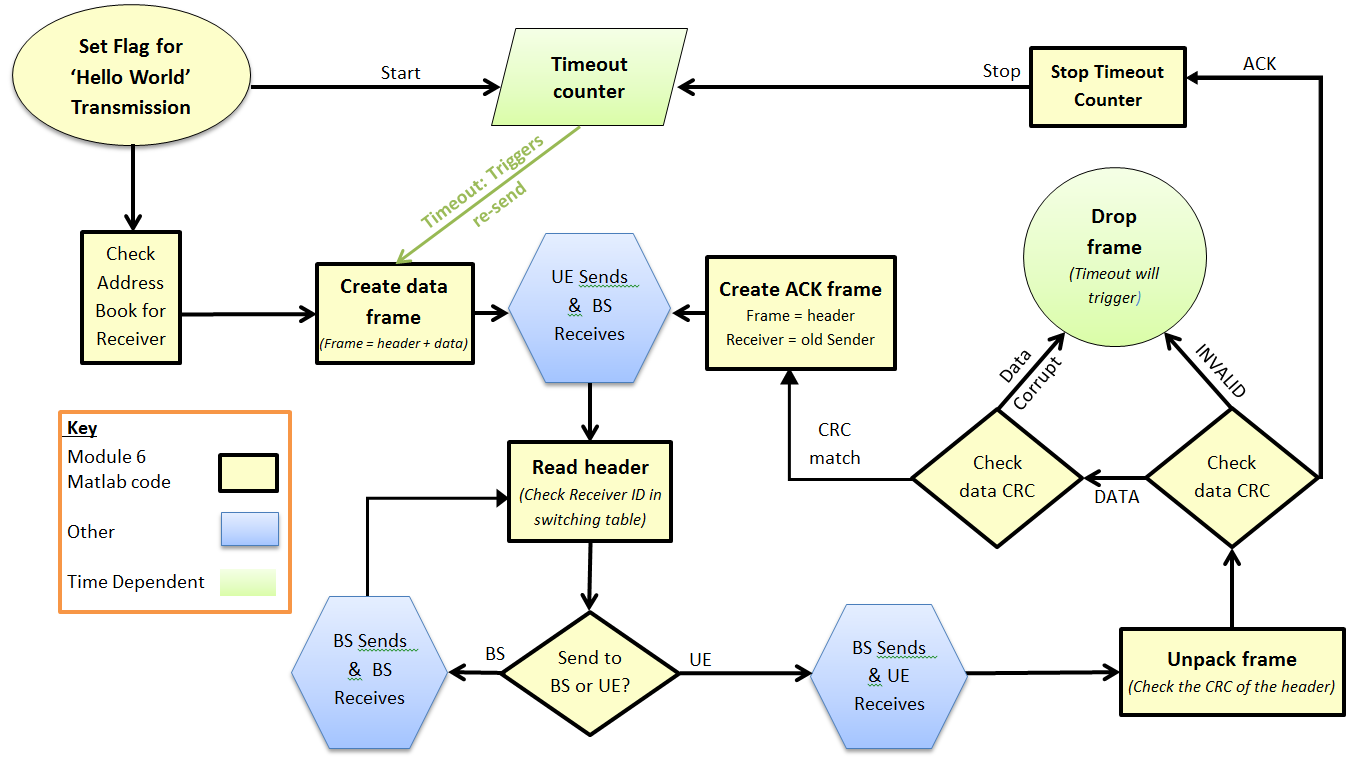
\includegraphics[width=0.8\textwidth]{State_Machine_yellow.PNG}
    \caption{State Machine of the transmission of a package }
    \label{fig:stateMachine}
\end{figure}

\subsection {The ACK response }
The ACK response should only be triggered by the transmission of correct data. We included the CRC of the data field as a section of the data frame so that the CRC can be used to check if the data has changed during any part of it's journey through the network. A data frame which fails the CRC check will have the same result as not receiving any frame at all or of receiving an INVALID frame, no ACK will be sent as seen in Figure \ref{stateMachine}. A correct CRC should trigger the UE to send a ACK with the rec

If there is no ACK received back from the UE that was sent a data frame, then that data frame will eventually have to be resent from the original UE to achieve transmission. The data frame should not be resent before the ACK has an appropriate amount of time to return. Depending on the position of each UE's timeslot in the transmission cycle and whether the UEs are within the same cell, the total time between the the transmission of the data frame and the reception of the ACK will vary greatly. Figure \ref{fig:ACKtimeshort} shows the shortest possible time between transmission and reception. Figure \ref{fig:ACKtimelong} shows the longest, the time increases by a factor of 2. 
\begin{figure}[ht]
    \centering
    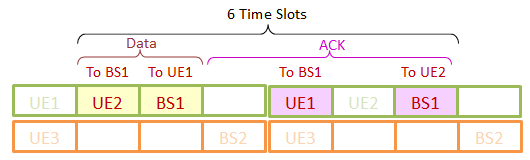
\includegraphics[width=0.8\textwidth]{ACK_timeout_short.PNG}
    \caption{Diagram of the shortest time between a UE transmitting a frame of data and receiving the corresponding ACK}
    \label{fig:ACKtimeshort}
\end{figure}

\begin{figure}[ht]
    \centering
    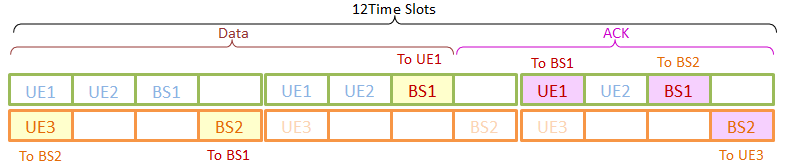
\includegraphics[width=0.8\textwidth]{ACK_timeout_long.PNG}
    \caption{Diagram of the longest time between a UE transmitting a frame of data and receiving the corresponding ACK}
    \label{fig:ACKtimelong}
\end{figure}



% so I am going to be describing the state machine essentially....was going to do this but I might go and write the intro frist to have a beter idea of what is going on.




\section{Frame Types descriptions}
%Renato
We created two frame type baaed on the needs of make a end to end communication.

\begin{description}
  \item[Data Frame] \hfill \\
  It is used to transmit a string message with the limit of 234 bytes. The encode of those bytes is using a ASCII standard. All the bits are order to left most significant bit.
	It is important to guaranteed the decoding of this string in the receiver don’t be machine depend. 
	
  \item[ACK Frame] \hfill \\
  It is the smallest package possible becuase it only have the header information because the data files is not transmitted. It make its transmission time smaller than any data frame. It is reused by Team 4 in their test. 
\end{description}

The frame object was used by other teams so three new types were defined and used by them.
\begin{description}
  \item[REQ Frame] \hfill \\
It is used by Team 4 to request a polling for all devices on the network. It was used by Team 4
	
  \item[Poll Frame] \hfill \\
 It is used by Team 4 to return the polling information of current device to requested polling. 
  \item[Table Frame] \hfill \\
 It is used by Team 5 to return the address table for all devices in the network.

\end{description} 

The frame type was a easy way to change the behavior of the receiving process based on the type.  
%RGB 253 254 202


